\documentclass[12pt]{Report}
\usepackage{graphicx}
\usepackage{listings}
\usepackage{listings}
\usepackage{verbatim} 
\begin{document}
\title{Assignment 4 : CS 751 }
\author{HARISH}

\maketitle

\section{Question 1}

\paragraph{ Using the pages from A3 that boilerpipe successfully processed, download those representations again and reprocess them with boilerpipe.\\ Document the time difference \\
Compute the Jaccard Distance x for each Pair of Pages for :Unique terms ,Bigrams,TriGrams\\ For each of 3 cases build a Cumulative Distribution Function that shows the percentage change on the x-axis and percentage of the population on y-axis\\ Give 3-4 examples illustrating the range of change that you have measured}

 

\subparagraph{Solution to Question1: \\}

I have used jusText library to remove HTML templates in Assignment 3 and 4. It removes headers, footers and navigation links from the page.\\
jusText was successful for pages that followed HTML standards. Pages which are properly organized .\\
 \\
I have written a code in python named "htmlnonhtml.py" which is located in "q1-A4" folder. This code removes boilerplate content for the links present in "responseAfterCurlCalls" located in "q1-A4" folder. \\

Only 6100 URIs were unique , out of this only for 1496 URIs boilerpipe sucessfully processed . Most of them are non-HTML skipped because of non content , Images on links , 404, 302 errors etc. \\

I have used the same pages from A3 for which boilerpipe was successfully processed. I have reprocessed those pages with boilerpipe and extracted the text files again for A4  \\

The time difference between A4 and A3 is \\

Time(A4)-Time(A3) : Time difference is 28 days March 30 to April 28


I have created two folders "A3-afterboilerplateTextFiles", "A4-afterboilerplatetextfiles" which is located inside "q1-A4" folder. These folders contains text files that were extracted after processing boilerpipe successfully for A3 and A4.\\\\

I have calculated Unique terms ,Bigrams , Trigrams for the text files located in the following folders :\\ \\
1)"A3-afterboilerplateTextFiles"  located inside "q1-A4" folder  \\
2)"A4-afterboilerplatetextfiles" located inside "q1-A4" folder \\

I have written a java code named "UniGram.java","BiGram.java", "TriGram.java"  located in "q1-A4" folder to extract unique terms, bigrams and trigrams respectively from  the text files . \\

I wrote a "jacarrdDistanceCalculator.py" code located inside "q1-A4" folder . This code reads the textual data generated for each pair of pages from A3 and A4 and calculates the jaccard distance for unique terms , bigrams and trigrams and saves them to an output file named "unijackardsorted.txt" , "bijacardsorted", "trijacardsorted" respectively. These files are located inside the folder "q1-A4" \\ \\

For each of the 3 cases (i.e., 1-,2-,3-grams ) I built a cumulative distribution function that shows percentage change on the x-axis and the percentage of population on the y-axis. \\ \\

Figure 1 ,Figure 2 , Figure 3 represents the Cumulative Distribution Function for Unigram , BiGram , TriGram respectively .  I have plotted the graph using R script . BiJacard.R , UniJacard.R , TriJacard.R are the scripts for generating Cumulative Distribution Function  graphs for Bigrams , UniGrams, Trigrams respectively . These are located inside "q1-A4" folder.\\

Following are the three examples illustrating the range of change measured \\

1) For this link "http://pinterest.com/pin/300896818829344973/" after successfully processing boilerpipe, there is a lot of change in textual content. Interesting part here is that, the unigram jaccard distance  for this link is "0.958333333333" where as for Bigram and TriGram jaccard distance is "1"\\


2) For this link "http://suba.me" after successfully processing boilerpipe , there is a little change in textual content. But, the jaccard distance for unigram , bigram and trigram are 0.0173611111111, 0.0138248847926, 0.0134831460674 respectively . Jaccard Distances are not same for unigram , bigram and trigram \\


3) For this link "http://twi.xsrv.jp/eot4j" after successfully processing boilerpipe, there is no change in the textual content. The Jaccard distances(1-gram, 2-gram, 3-gram) for these pair of pages from A3  and A4 is 0.\\
 




\section{Question 2\\}

\paragraph{from Q1 (A4), download all TimeMaps(including TimeMaps with 404 responses, i.e. empty or null TimeMaps) \\ Upload all TimeMaps to github\\ Build a CDF for number of mementos for each original URI i.e., x-axis = number of mementos , y-axis = number of links \\\\ }

\subparagraph{Solution to Question2: \\}
I have written a code "getURLData.py" which is located inside the "q2-A4" folder. This code reads "urlStatusAfterCurlCalls" file which contains the URIs. This is located in "q2-A4" .\\ I have used  "http://labs.mementoweb.org/timemap/link/" to get the mementos for each URI. This codes saves all the TimeMaps for all the 10000 links. These are saved inside "q2-A4/timemaps/" folder .This list includes the null time maps as well.\\

After collecting the mementos for each URI , I have written a python script named "mementocount.py" which extracts the count of mementos per each URI and saves it to "timemapsCount.txt" file which is located inside "q2-A4" folder.\\
 

Figure 4 shows the cumulative distribution function for all the count of mementos. I have written a R script named "cdfformemntos.R" located inside "q2-A4".  Most of the URIs have zero mementos. \\


\section{Question 3\\}

\paragraph{Using 20 links that have TimeMaps - \\ -With>=20 mementos\\-Have existed greater than equal to 2 years i.e., Memento-Datetime of "first memento" is April XX, 2013 or older\\ -Note : select from Q1/Q2  links , else choose them by hand \\ For each link , create a graph that shows Jaccard Distance, relative to the first memnto, through time\\-x-axis : continuous time ,y-axis: Jaccard Distance relative to the first memento \\\\ }


\subparagraph{Solution to Question3: \\}

I have chosen 20 links by hand  that satisfies the question criteria. I have saved these files into "final20links.txt" which is located inside "q3-A4" folder.\\
I have written a code "getURLData.py" located inside "q3-A4" folder . This code reads "final20links.txt" and extracts the mementos links for each URI in the list in json format with the help of "http://labs.mementoweb.org/timemap/json/" . \\

I have saved all of these files with '.json' extension.  I have written a python script with name "html-non-html.py" located in "q3-A4" folder which reads each json file in the directory  ("q3-A4" folder) and iterates through each memento present in the  list (json Array)  for each URI and applies boilerpipe to each link.
Most of the links were not successfully processed after applying boilerpipe. For the URIs for which boilerpipe successfully processed, I have calculated the Jaccard distance relative to first memento.\\

I have written a Rscript named "JDRelativetofirstMemento.R" which is located in "q3-A4" folder \\

Figure 5- Figure 18 shows Jaccard Distance relative to first memento.



\section{Question 4\\}

\paragraph{Choose a news-related event\\ UseTwarc.py to collect 1000 tweets , every day for 5 different days \\For each day:\\ - Create a wall \\ - Build a tag/word cloud for each day \\ - Create a map using GeoJSON and Github\\ Discuss in detail lessons learned , experiences , etc\\}

\subparagraph{Solution to Question4: (Figure 19 to Figure 33) \\\\}
Firstly, I have generated a consumer key, consumer secret key, access token and access-secret token.\\
 I have collected 1000 tweets, every day for 5 different days.\\
I have written a script(using above mentioned keys)  named "twarc1.py" located inside folder "q4-A4". I have extracted the tweets on "AppleWatch" tag. I have saved these 1000 tweets daily with ".json" extension .\\
The files are located inside the folder "q4-A4".Following are the files I have extracted on a daily basis for 5 different days\\ 

tweets25th.json \\
  tweets26th.json \\
  tweets27th.json \\
  tweets28th.json \\
  tweets30th.json \\

I have copied all of these inside "twarc-master/utils/".
Then, I have given above json files as an input to wall.py to create Wall on daily basis. It gave me output wall with '.html' extension. All of these output files are stored inside "q4-A4/wall/" folder. The wall basically gives the information of all the tweets that are related to "Applewatch" for each day. 



I have given above files as an input to word.py to create word cloud on daily basis. It gave me output wordcloud files with '.html' extension.
The files are located inside the folder "q4-A4/wordcloud/". Word Cloud mainly enlarges mostly used word from the tweets . The frequency of the words is directly proportional to the Size of the word visible in the output wordcloud file.

I have also given above json files as an input to tweets.geojson to get geo coordinates from the tweets.
 I have uploaded the geojson files located inside 'q4-A4/geojson/'  .After uploading these geojson files , github shows the map with markers located using "geojson coordinates".  
 

\begin{figure}[ht]    
    \begin{center}
        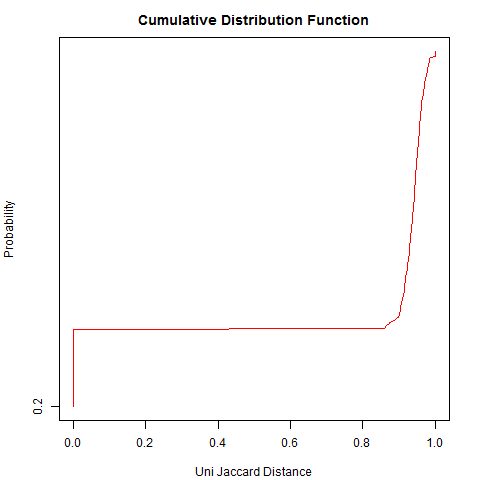
\includegraphics[scale=0.60]{unigram.png}
        \caption{CDF for Unigram Jaccard Distance }
        \label{UniGram Jaccard Distance}
    \end{center}
\end{figure}
\newpage
 
 
\begin{figure}[ht]    
    \begin{center}
        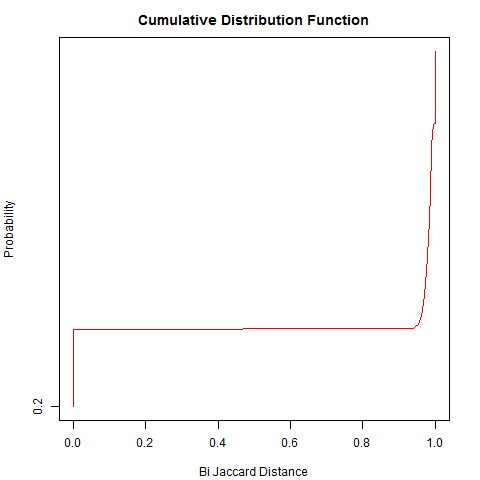
\includegraphics[scale=0.60]{bigram.png}
        \caption{CDF for Bigram Jaccard Distance }
        \label{BiGram Jaccard Distance}
    \end{center}
\end{figure}
\newpage


\begin{figure}[ht]    
    \begin{center}
        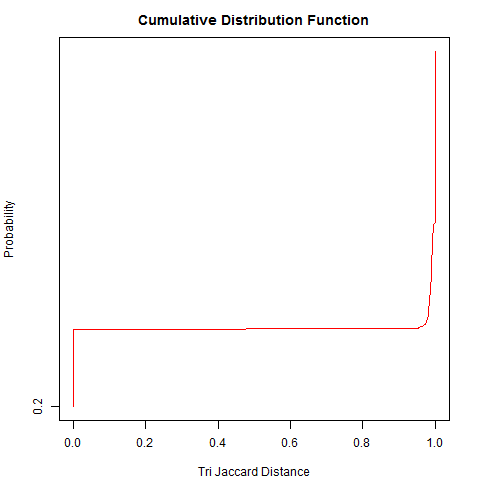
\includegraphics[scale=0.60]{trigram.png}
        \caption{CDF for Trigram Jaccard Distance }
        \label{TriGram Jaccard Distance}
    \end{center}
\end{figure}
\newpage

\begin{figure}[ht]    
    \begin{center}
        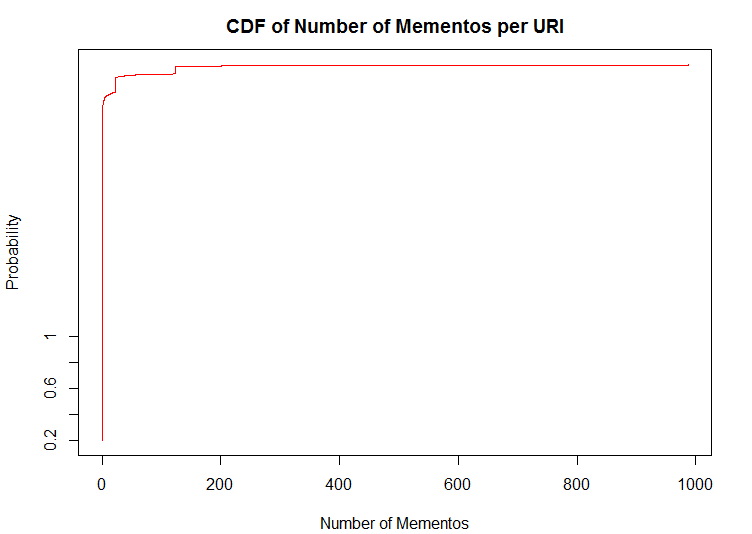
\includegraphics[scale=0.60]{NumberOfMementoS.png}
        \caption{CDF for number of mementos for each original URI }
        \label{CDF for number of mementos for each original URI }
    \end{center}
\end{figure}
\newpage

 
 \begin{figure}[ht]    
    \begin{center}
        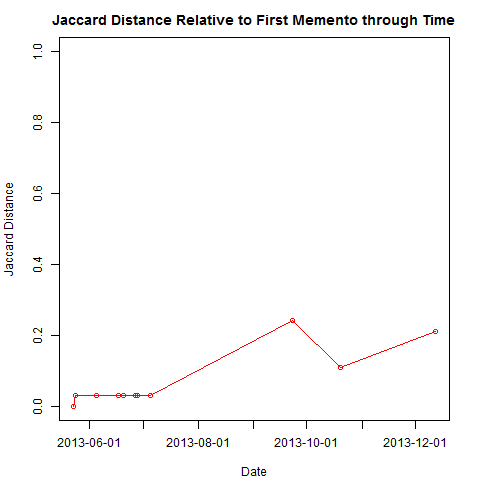
\includegraphics[scale=0.60]{link1.png}
        \caption{Jaccard Distance Relative to First Memento }
        \label{Jaccard Distance Relative to First Memento}
    \end{center}
\end{figure}
\newpage
 
 
\begin{figure}[ht]    
    \begin{center}
        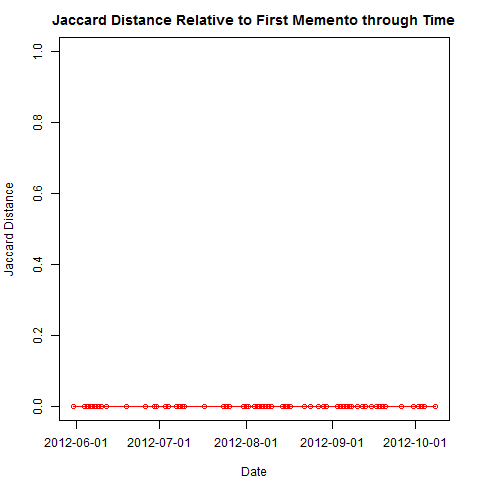
\includegraphics[scale=0.60]{link2.png}
        \caption{Jaccard Distance Relative to First Memento }
        \label{Jaccard Distance Relative to First Memento}
    \end{center}
\end{figure}
\newpage 

\begin{figure}[ht]    
    \begin{center}
        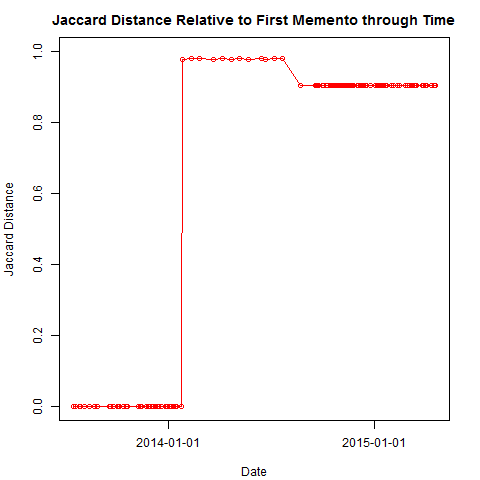
\includegraphics[scale=0.60]{link3.png}
        \caption{Jaccard Distance Relative to First Memento }
        \label{Jaccard Distance Relative to First Memento}
    \end{center}
\end{figure}
\newpage

 
 \begin{figure}[ht]    
    \begin{center}
        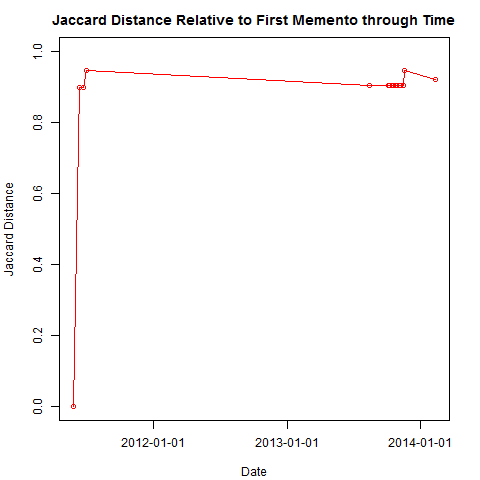
\includegraphics[scale=0.60]{link4.png}
        \caption{Jaccard Distance Relative to First Memento }
        \label{Jaccard Distance Relative to First Memento}
    \end{center}
\end{figure}
\newpage


\begin{figure}[ht]    
    \begin{center}
        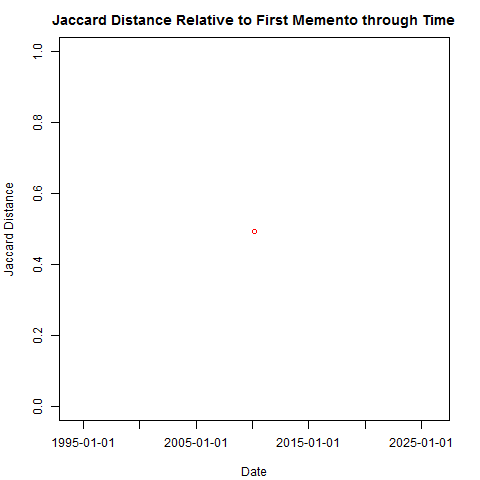
\includegraphics[scale=0.60]{link5.png}
        \caption{Jaccard Distance Relative to First Memento }
        \label{Jaccard Distance Relative to First Memento}
    \end{center}
\end{figure}
\newpage


\begin{figure}[ht]    
    \begin{center}
        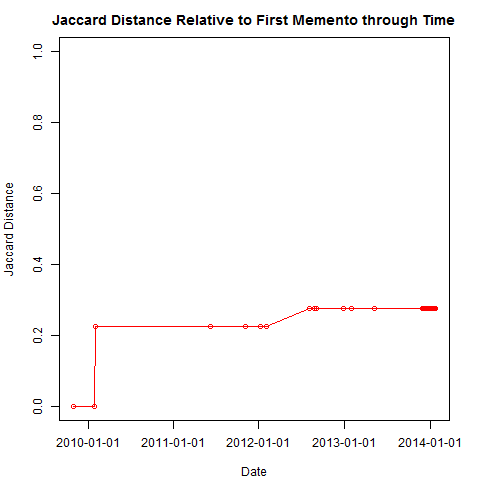
\includegraphics[scale=0.60]{link6.png}
        \caption{Jaccard Distance Relative to First Memento }
        \label{Jaccard Distance Relative to First Memento}
    \end{center}
\end{figure}
\newpage

\begin{figure}[ht]    
    \begin{center}
        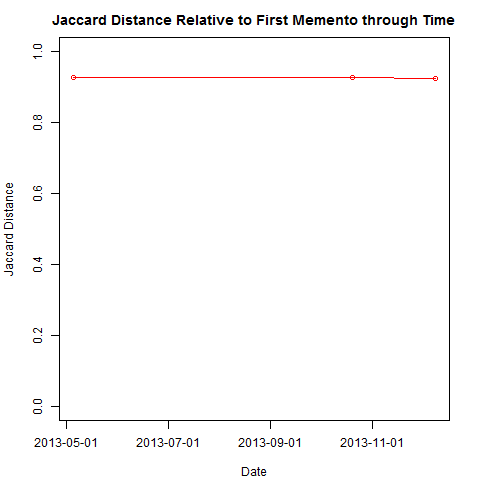
\includegraphics[scale=0.60]{link7.png}
        \caption{Jaccard Distance Relative to First Memento }
        \label{Jaccard Distance Relative to First Memento}
    \end{center}
\end{figure}
\newpage


\begin{figure}[ht]    
    \begin{center}
        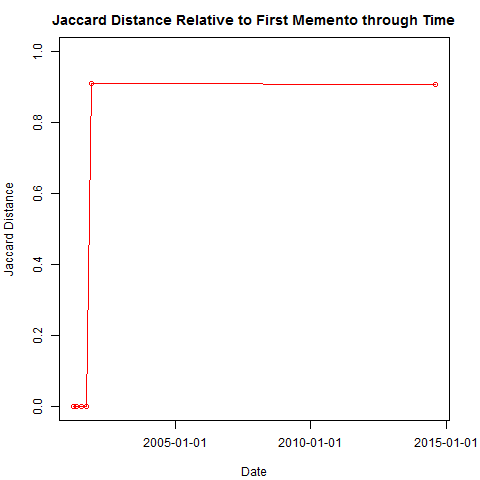
\includegraphics[scale=0.60]{link8.png}
        \caption{Jaccard Distance Relative to First Memento }
        \label{Jaccard Distance Relative to First Memento}
    \end{center}
\end{figure}
\newpage

\begin{figure}[ht]    
    \begin{center}
        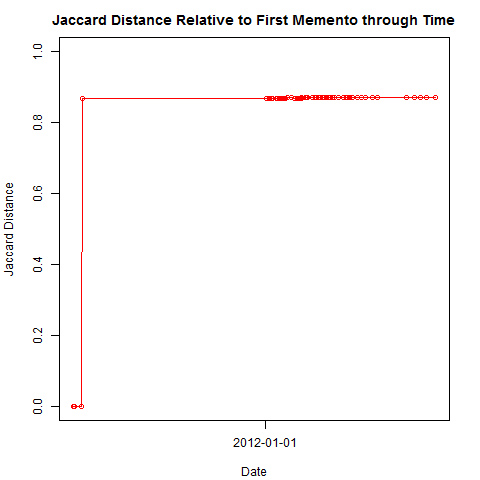
\includegraphics[scale=0.60]{link10.png}
        \caption{Jaccard Distance Relative to First Memento }
        \label{Jaccard Distance Relative to First Memento}
    \end{center}
\end{figure}
\newpage

\begin{figure}[ht]    
    \begin{center}
        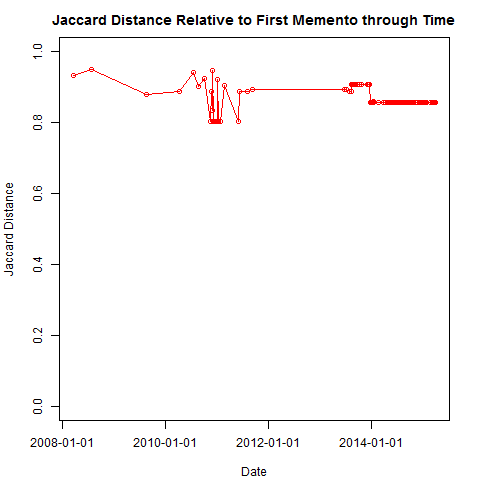
\includegraphics[scale=0.60]{link11.png}
        \caption{Jaccard Distance Relative to First Memento }
        \label{Jaccard Distance Relative to First Memento}
    \end{center}
\end{figure}
\newpage

\begin{figure}[ht]    
    \begin{center}
        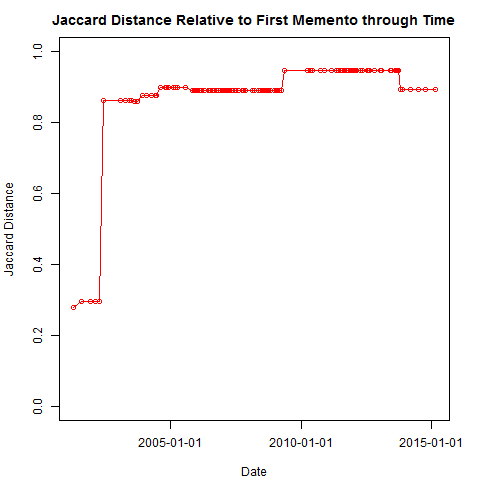
\includegraphics[scale=0.60]{link14.png}
        \caption{Jaccard Distance Relative to First Memento }
        \label{Jaccard Distance Relative to First Memento}
    \end{center}
\end{figure}
\newpage


\begin{figure}[ht]    
    \begin{center}
        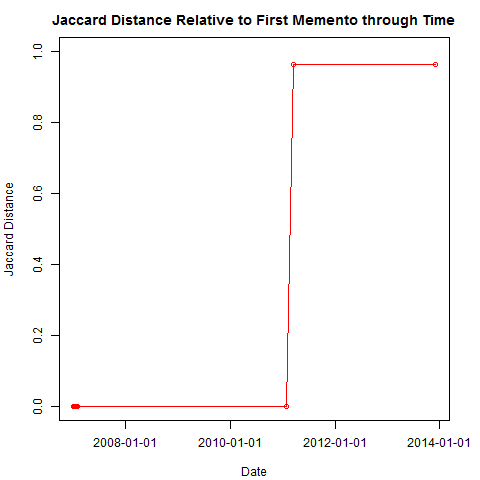
\includegraphics[scale=0.60]{link15.png}
        \caption{Jaccard Distance Relative to First Memento }
        \label{Jaccard Distance Relative to First Memento}
    \end{center}
\end{figure}
\newpage

\begin{figure}[ht]    
    \begin{center}
        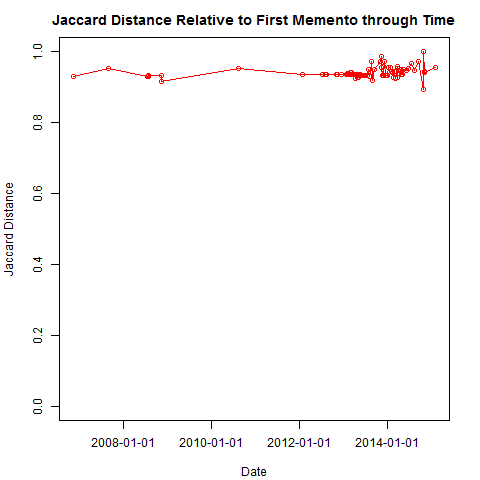
\includegraphics[scale=0.60]{link16.png}
        \caption{Jaccard Distance Relative to First Memento }
        \label{Jaccard Distance Relative to First Memento}
    \end{center}
\end{figure}
\newpage

\begin{figure}[ht]    
    \begin{center}
        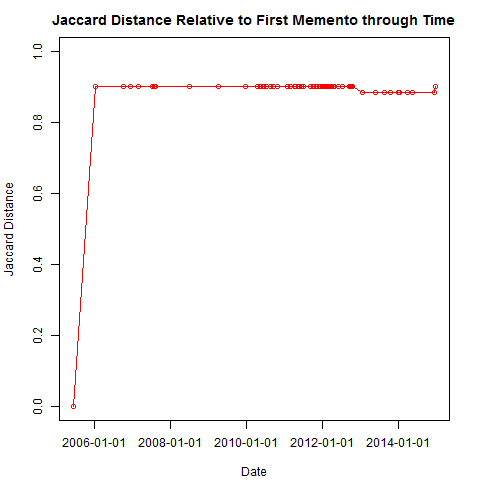
\includegraphics[scale=0.60]{link18.png}
        \caption{Jaccard Distance Relative to First Memento }
        \label{Jaccard Distance Relative to First Memento}
    \end{center}
\end{figure}
\newpage


\begin{figure}[ht]    
    \begin{center}
        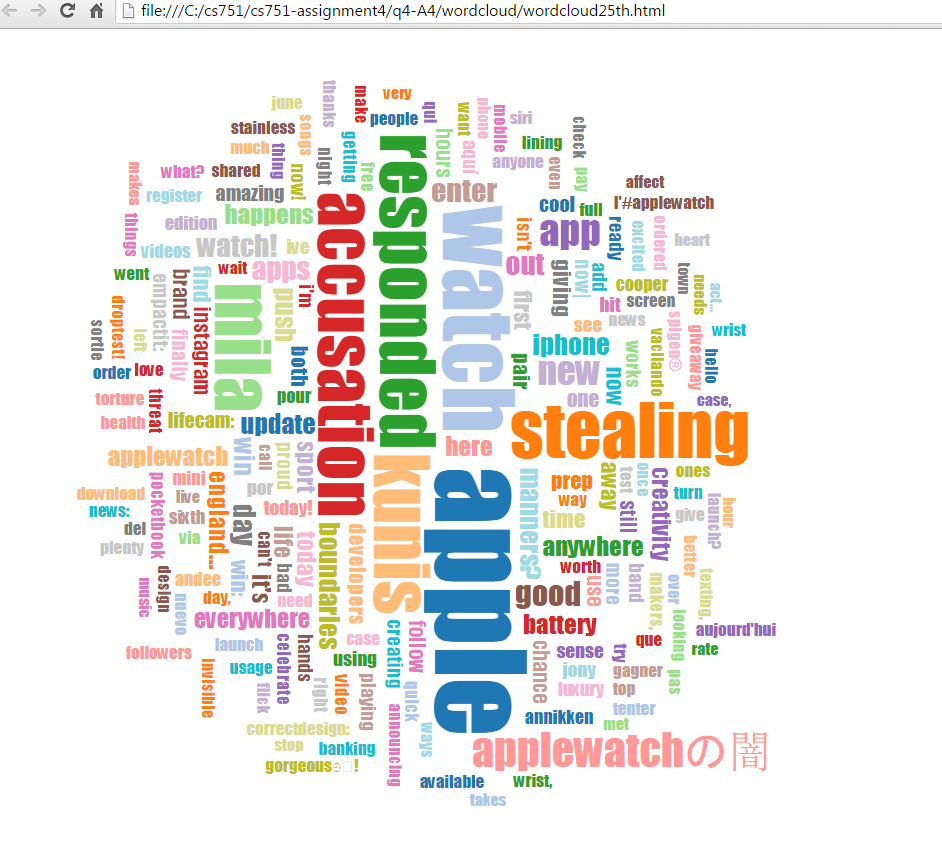
\includegraphics[scale=0.60]{word25th.png}
        \caption{WordCloud for Event "Apple Watch" on 25th March }
        \label{WordCloud for Event "Apple Watch" on 25th March}
    \end{center}
\end{figure}


\begin{figure}[ht]    
    \begin{center}
        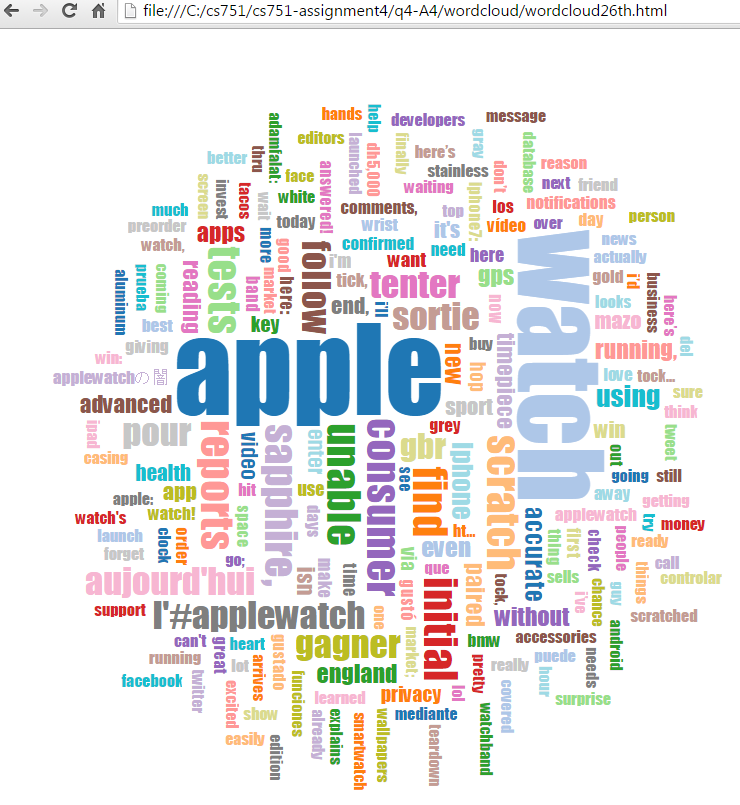
\includegraphics[scale=0.60]{word26th.png}
        \caption{WordCloud for Event "Apple Watch" on 26th March }
        \label{WordCloud for Event "Apple Watch" on 26th March}
    \end{center}
\end{figure}

\begin{figure}[ht]    
    \begin{center}
        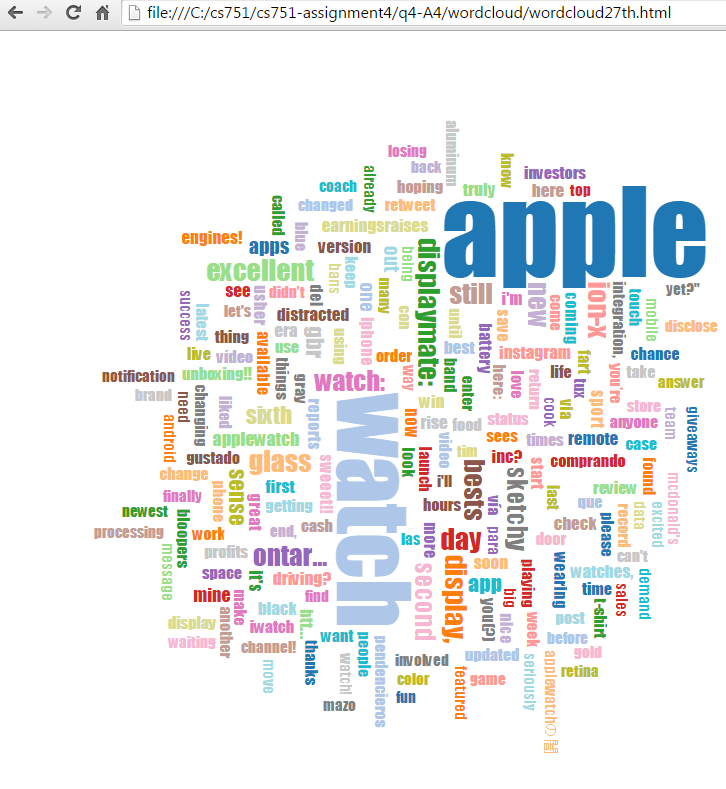
\includegraphics[scale=0.60]{word27th.png}
        \caption{WordCloud for Event "Apple Watch" on 27th March }
        \label{WordCloud for Event "Apple Watch" on 27th March}
    \end{center}
\end{figure}

\begin{figure}[ht]    
    \begin{center}
        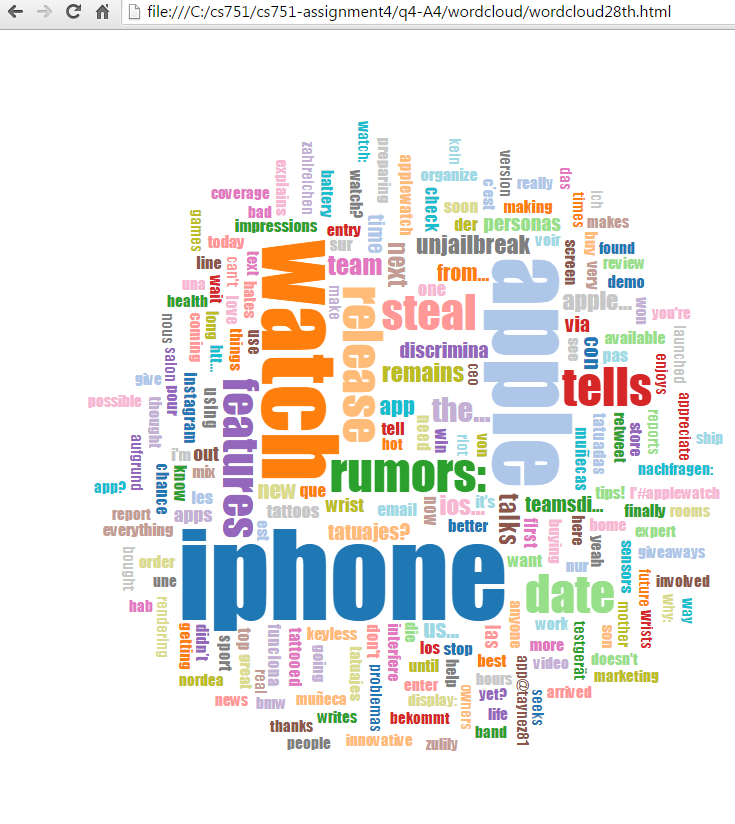
\includegraphics[scale=0.60]{word28th.png}
        \caption{WordCloud for Event "Apple Watch" on 28th March }
        \label{WordCloud for Event "Apple Watch" on 28th March}
    \end{center}
\end{figure}


\begin{figure}[ht]    
    \begin{center}
        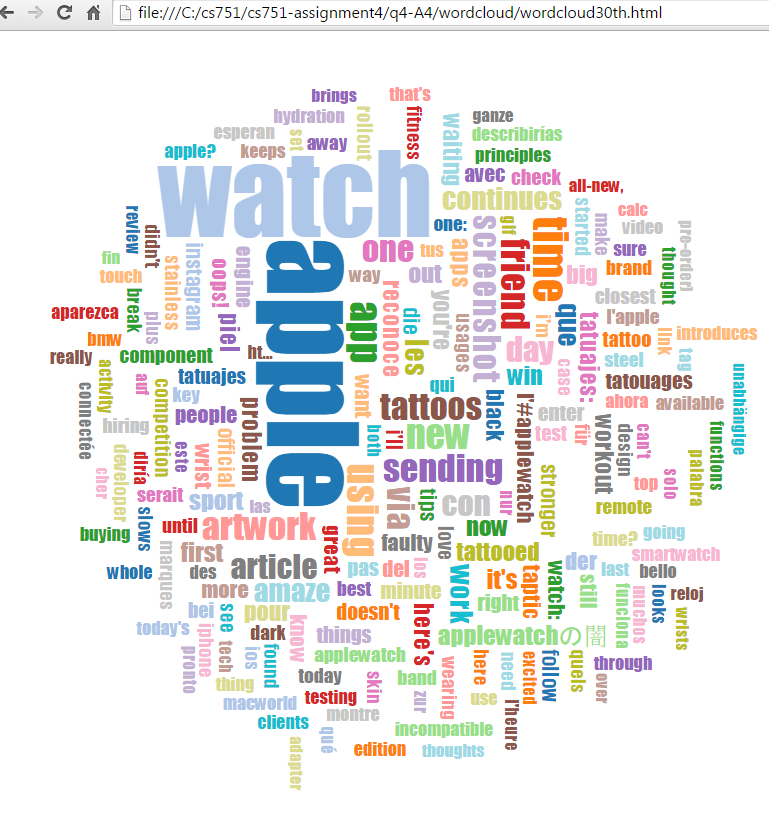
\includegraphics[scale=0.60]{word30th.png}
        \caption{WordCloud for Event "Apple Watch" on 30th March }
        \label{WordCloud for Event "Apple Watch" on 30th March}
    \end{center}
\end{figure}

\begin{figure}[ht]    
    \begin{center}
        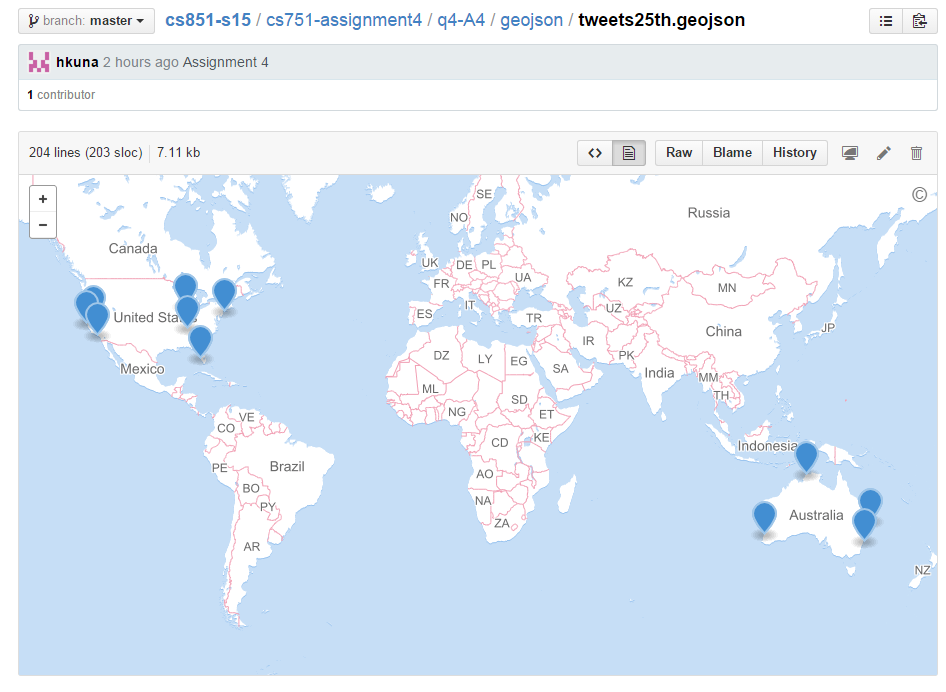
\includegraphics[scale=0.60]{geojson25th.png}
        \caption{Geo-Coordinates for Event "Apple Watch" on 25th March }
        \label{Geo-Coordinates for Event "Apple Watch" on 25th March}
    \end{center}
\end{figure}

\begin{figure}[ht]    
    \begin{center}
        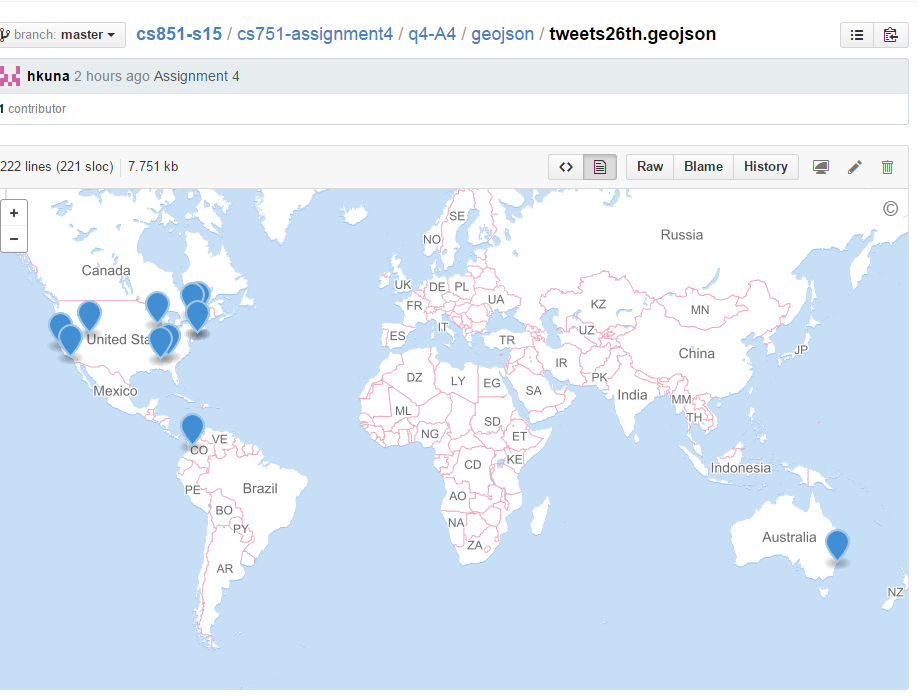
\includegraphics[scale=0.60]{geojson26th.png}
        \caption{Geo-Coordinates for Event "Apple Watch" on 26th March }
        \label{Geo-Coordinates for Event "Apple Watch" on 26th March}
    \end{center}
\end{figure}


\begin{figure}[ht]    
    \begin{center}
        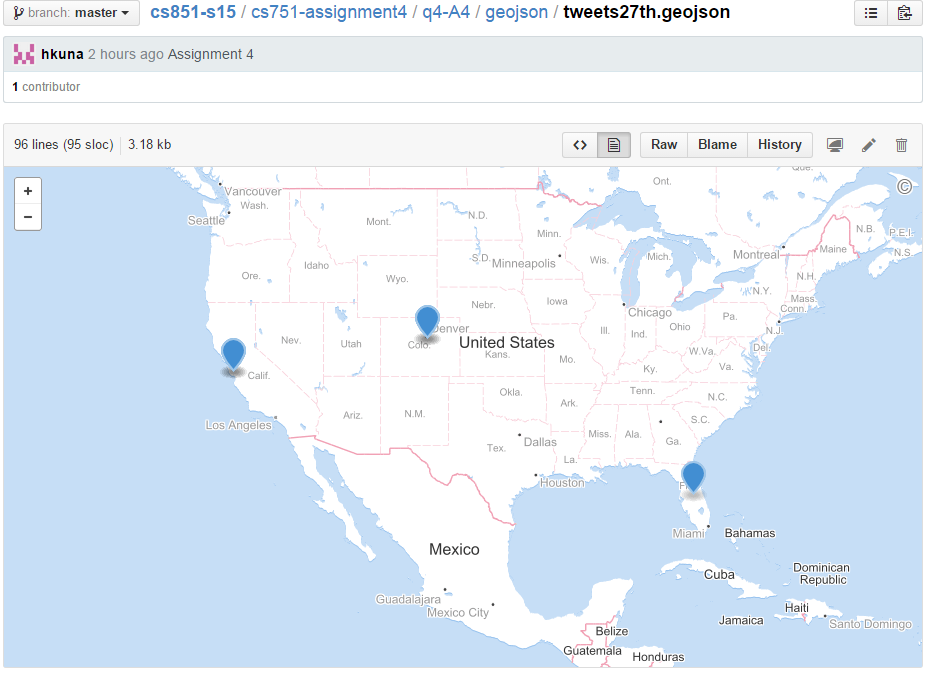
\includegraphics[scale=0.60]{geojson27th.png}
        \caption{Geo-Coordinates for Event "Apple Watch" on 27th March }
        \label{Geo-Coordinates for Event "Apple Watch" on 27th March}
    \end{center}
\end{figure}

\begin{figure}[ht]    
    \begin{center}
        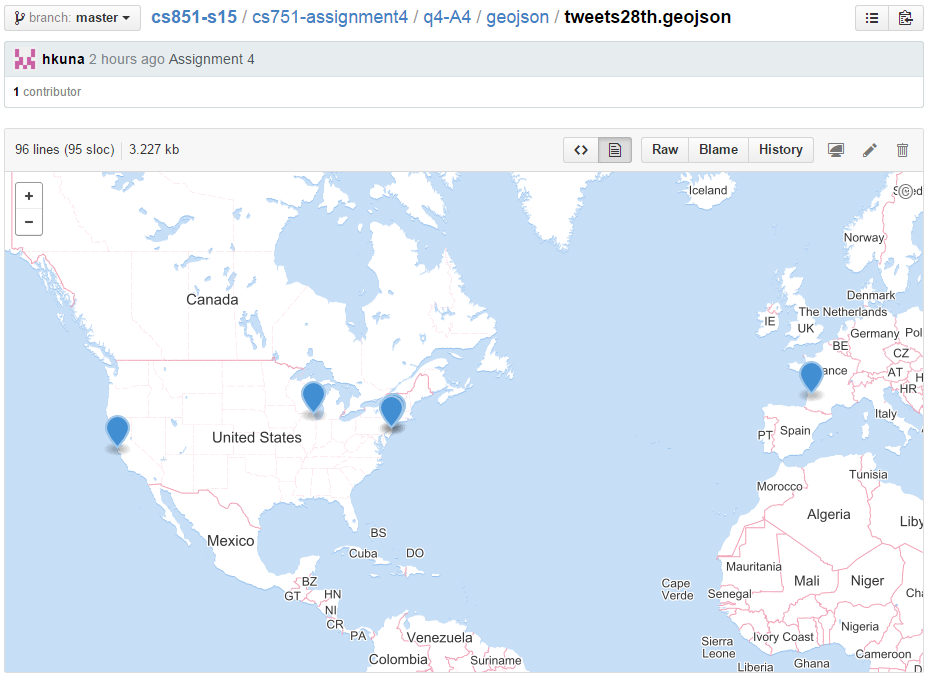
\includegraphics[scale=0.60]{geojson28th.png}
        \caption{Geo-Coordinates for Event "Apple Watch" on 28th March }
        \label{Geo-Coordinates for Event "Apple Watch" on 28th March}
    \end{center}
\end{figure}

\begin{figure}[ht]    
    \begin{center}
        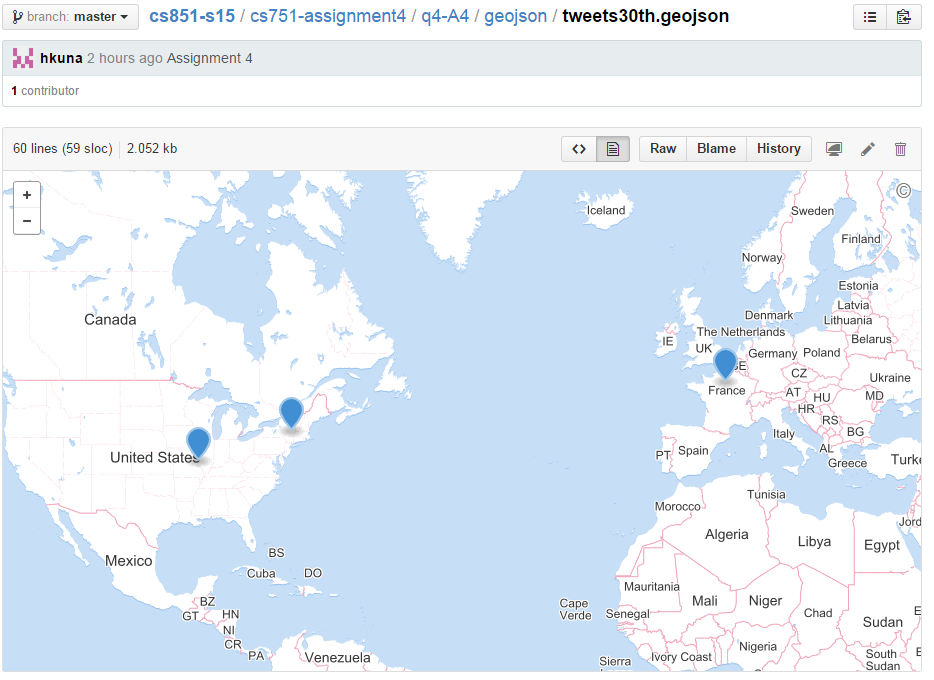
\includegraphics[scale=0.60]{geojson30th.png}
        \caption{Geo-Coordinates for Event "Apple Watch" on 30th March }
        \label{Geo-Coordinates for Event "Apple Watch" on 30th March}
    \end{center}
\end{figure}

\begin{figure}[ht]    
    \begin{center}
        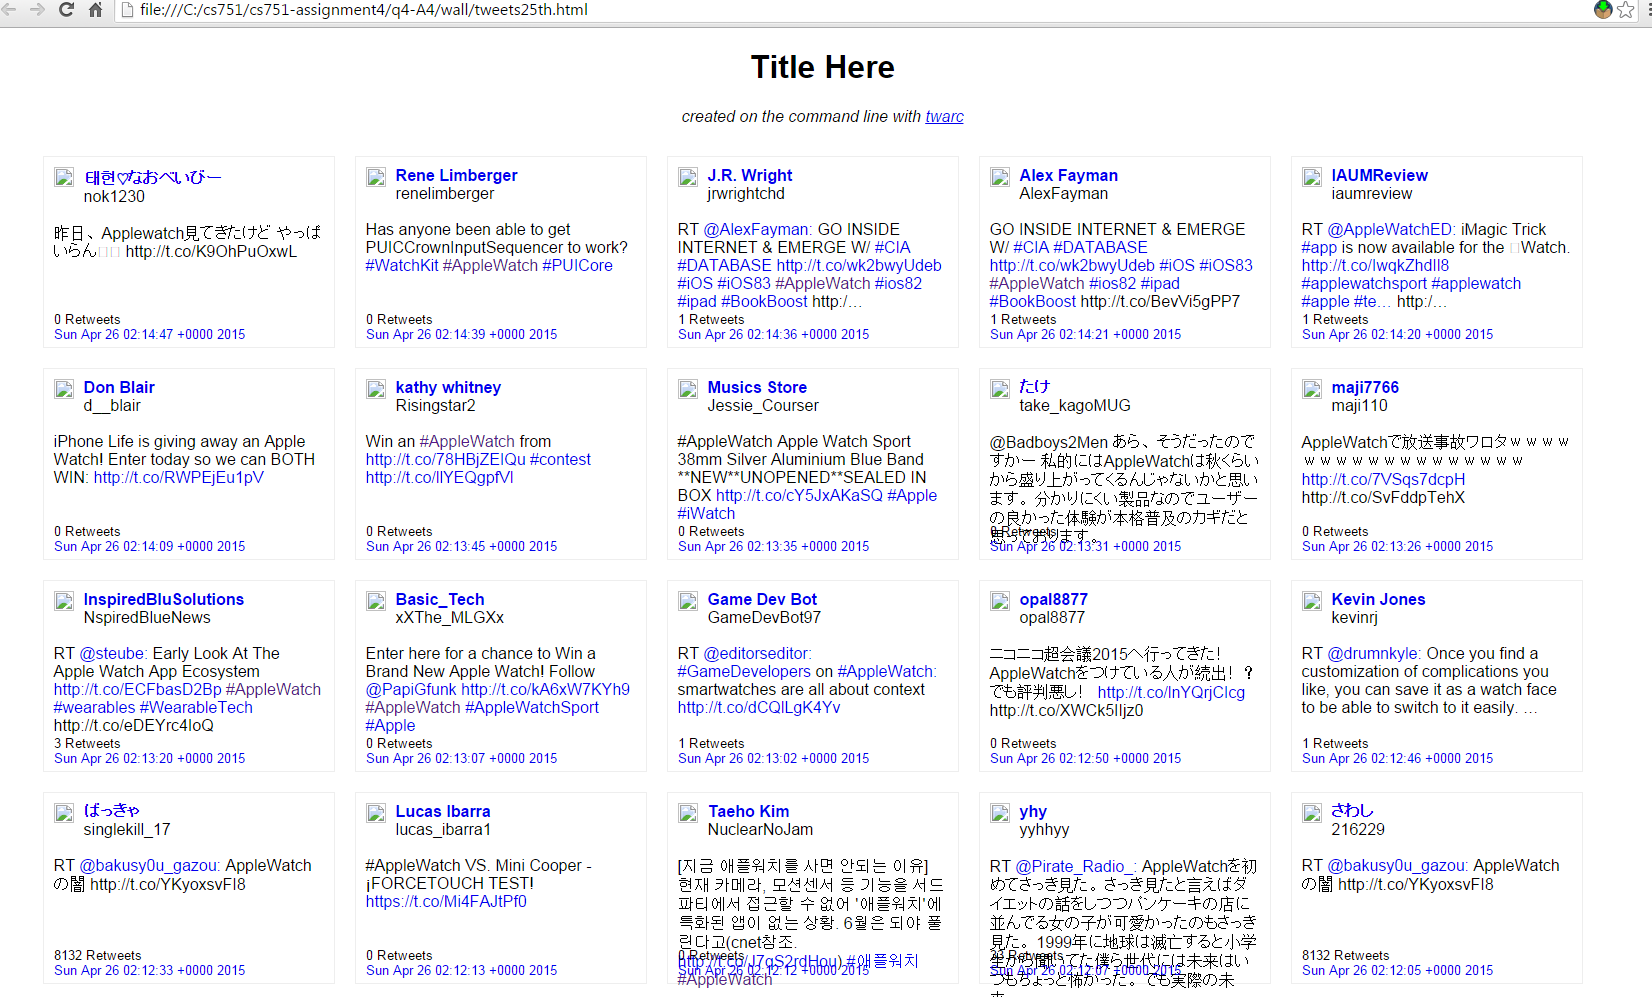
\includegraphics[scale=0.60]{wall25th.png}
        \caption{Wall for Event "Apple Watch" on 25th March }
        \label{Wall for Event "Apple Watch" on 25th March}
    \end{center}
\end{figure}


\begin{figure}[ht]    
    \begin{center}
        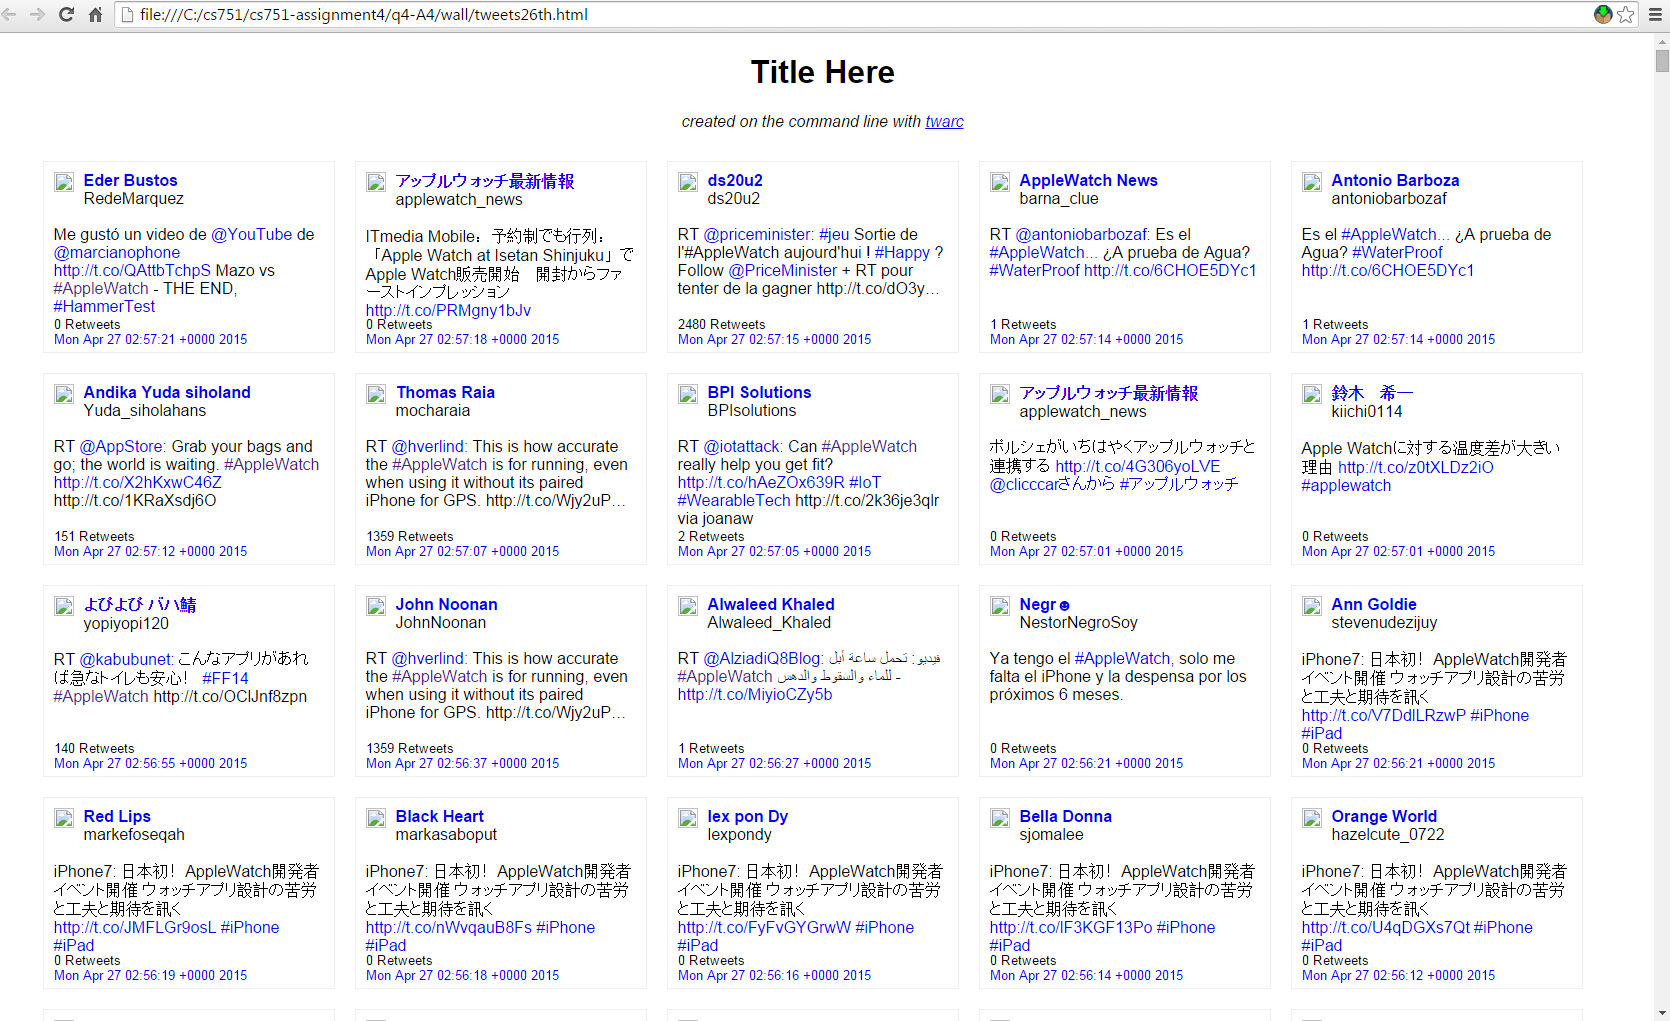
\includegraphics[scale=0.60]{wall26th.png}
        \caption{Wall for Event "Apple Watch" on 26th March }
        \label{Wall for Event "Apple Watch" on 26th March}
    \end{center}
\end{figure}

\newpage




\begin{figure}[ht]    
    \begin{center}
        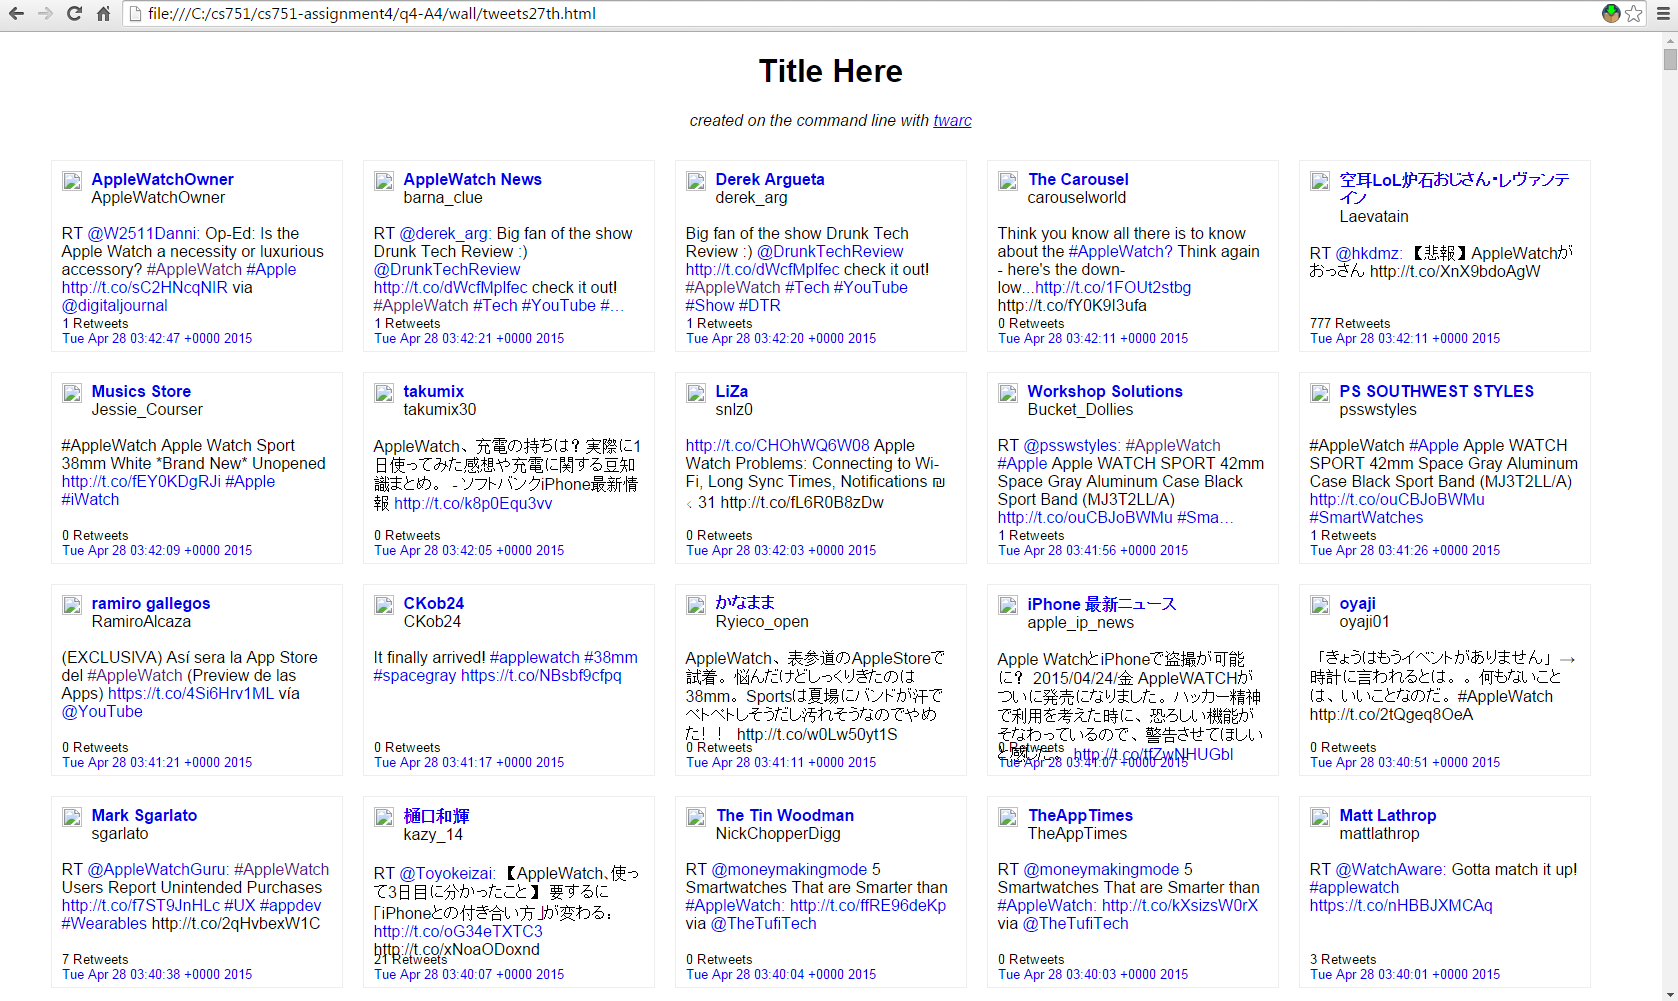
\includegraphics[scale=0.60]{wall27th.png}
        \caption{Wall for Event "Apple Watch" on 27th March }
        \label{Wall for Event "Apple Watch" on 27th March}
    \end{center}
\end{figure}



\begin{figure}[ht]    
    \begin{center}
        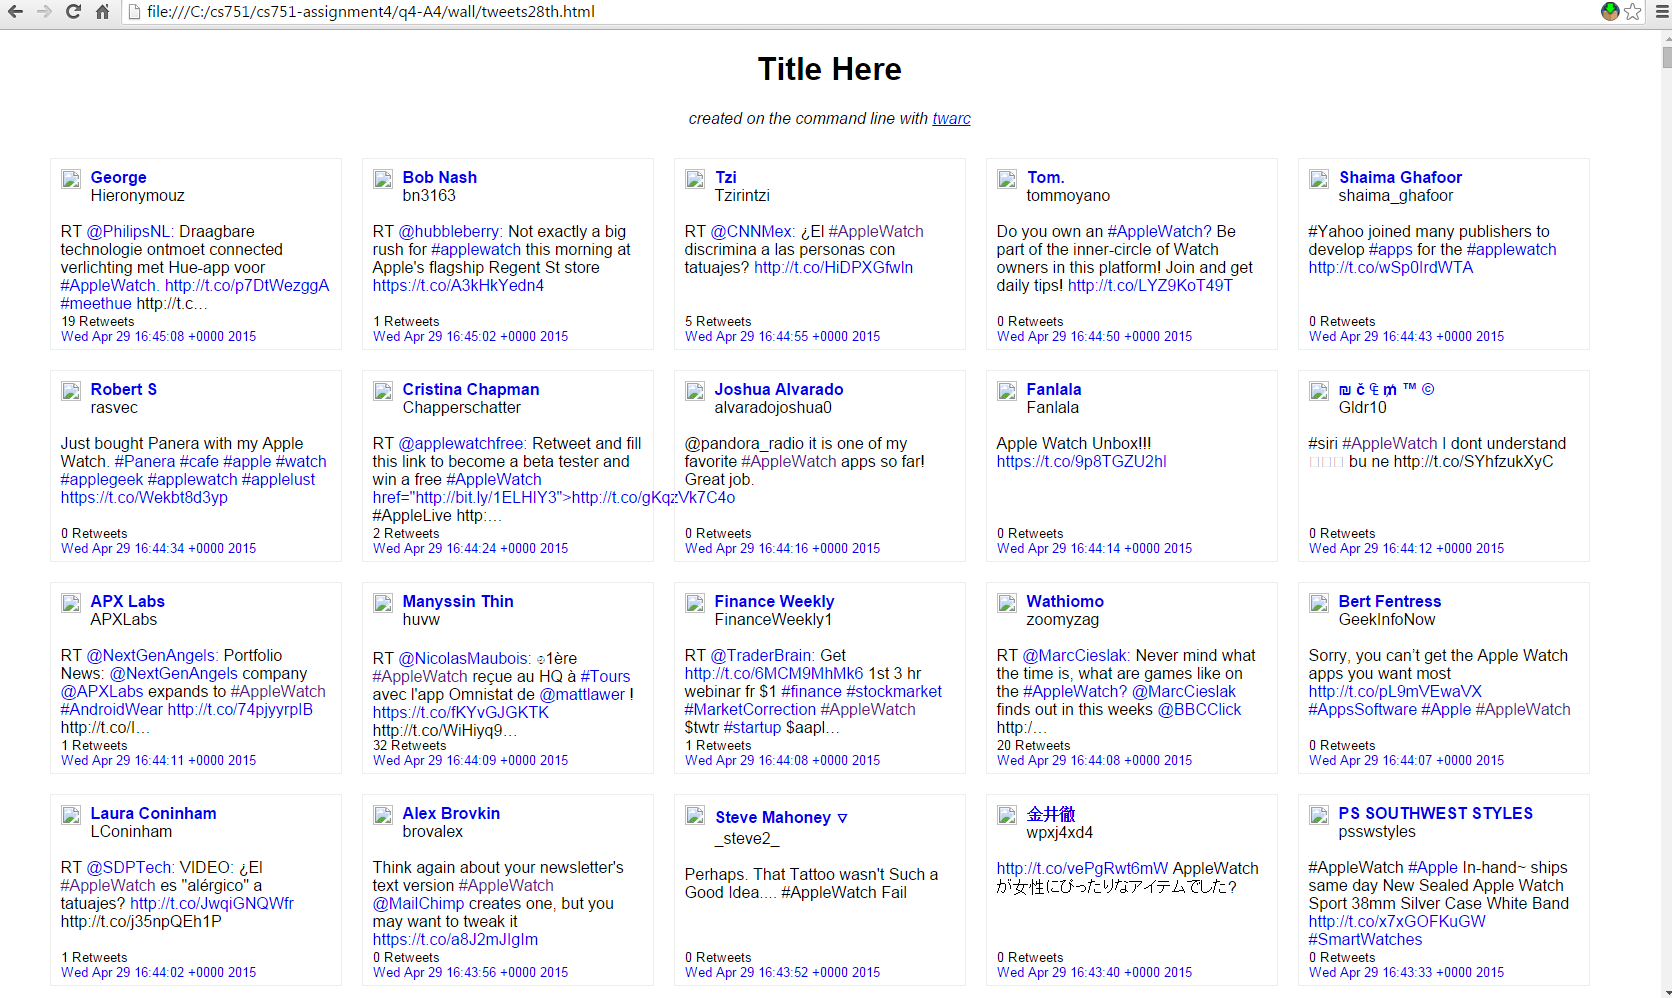
\includegraphics[scale=0.60]{wall28th.png}
        \caption{Wall for Event "Apple Watch" on 28th March }
        \label{Wall for Event "Apple Watch" on 28th March}
    \end{center}
\end{figure}



\begin{figure}[ht]    
    \begin{center}
        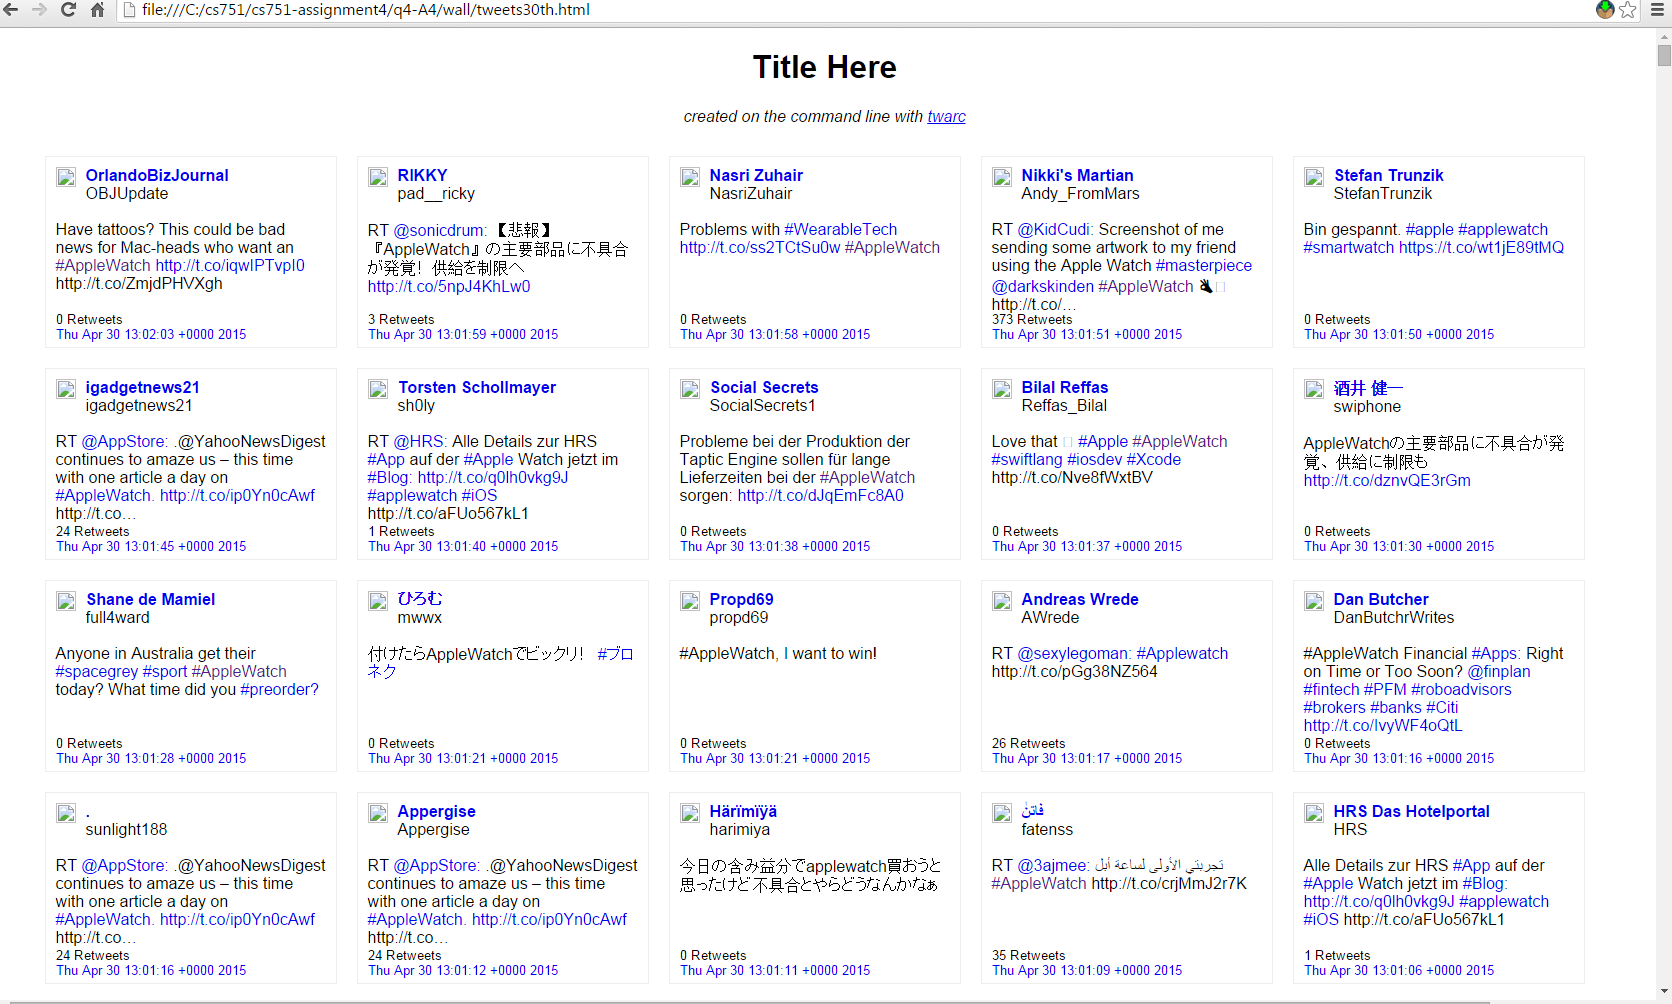
\includegraphics[scale=0.60]{wall30th.png}
        \caption{Wall for Event "Apple Watch" on 30th March }
        \label{Wall for Event "Apple Watch" on 30th March}
    \end{center}
\end{figure}

\bibliographystyle{plain}
\bibliography{bib4}
\nocite{*}


\end{document}


